\part{数学知识}

\chapter{线性代数基础}

本章的主要内容是对计算机图形学中的线性代数知识进行讲解 (或者说复习) . 

\section{向量}

向量指的是\textbf{具有大小 (Magnitude) 和方向 (Direction) 量}. 在物理学中也称为矢量. 向量的表示通常使用小写字母上面加上向右的箭头$\rightarrow$表示, 例如$\overrightarrow{a}$; 或者使用粗体的小写字母表示, 例如$\textbf{a}$. 

向量具有\textbf{平移不变形}. 向量只与大小和方向有关系, 和向量的起点和终点没有关系. 向量也只包含两个属性: \textbf{大小}和\textbf{方向}. 

对于空间中的两个点$A$和$B$, 从$A$到$B$的向量可以表示为$\overrightarrow{AB}$, 计算方法为$\overrightarrow{AB}=B-A$. 

\subsection{向量归一化}

向量的大小 (长度) 称为向量的模 (norm) , 一般记作$||\overrightarrow{a}||$. 

单位向量 (Unit vector) 指的是\textbf{模为1的向量}. 单位向量的计算公式为: 
\begin{equation}
\hat{a}=\frac{\overrightarrow{a}}{\big||\overrightarrow{a}|\big|}
\end{equation}

单位向量的长度为$1$, 一般只用来表示方向. 

\subsection{向量求和}
向量的求和可以用两种法则: \textbf{平行四边形法则}或者\textbf{三角形法则}. 

\begin{figure}[H]
  \centering
  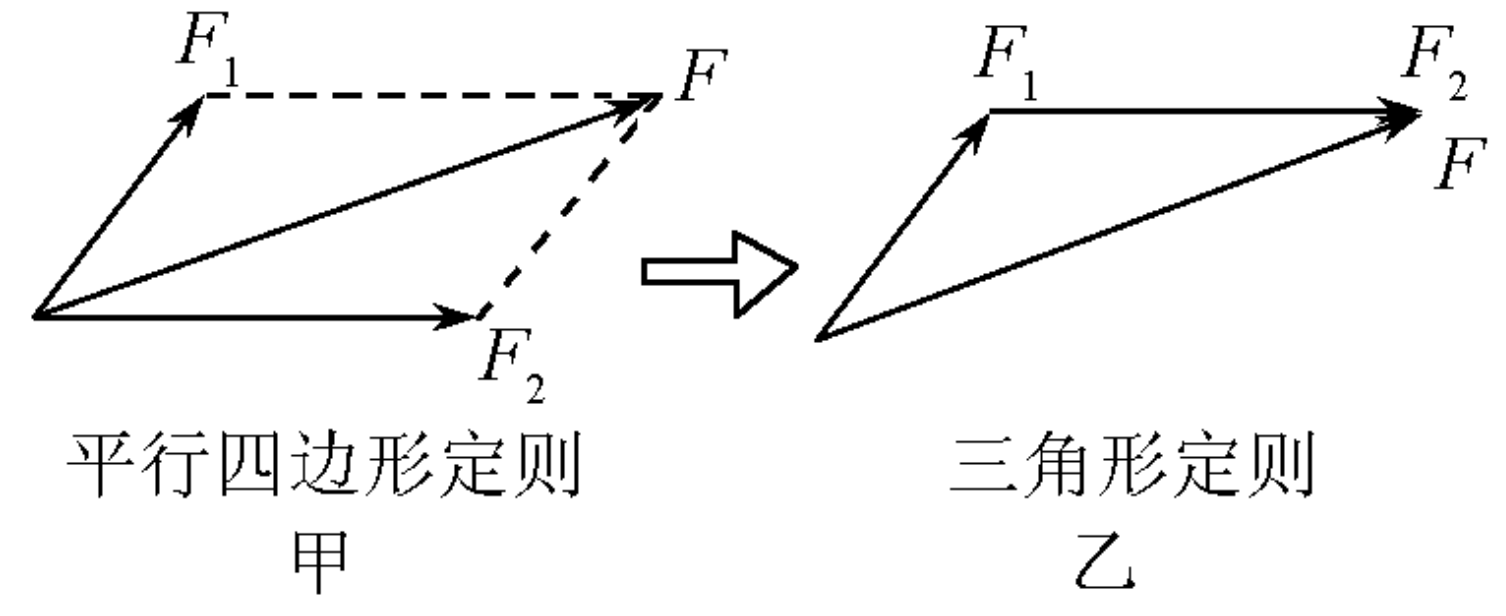
\includegraphics[scale=.3]{vectoradd.png}
  \caption{平行四边形法则与三角形法则}
  \label{fig:vectoradd}
\end{figure}

两个向量相加时, 以表示这两个向量的线段为邻边作平行四边形, 这两个邻边之间的对角线就代表向量和的大小和方向, 这就叫做\textbf{平行四边形定则 (Parallelogram law) }. 

\textbf{三角形法则 (Triangle law) }是指两个向量, 将一个向量的起点移动到另一个向量的终点时, 向量和为从未移动向量的起点指向所移动向量的终点的向量. 三角形法则适用于多个向量求和, 只需要将向量按照相加顺序依次首尾排列, 第一个向量的起点指向最后一个向量的终点的向量就是求和的结果. 

在代数上, 对于在笛卡尔坐标系中定义的向量, 向量求和可以简化为求向量各个对应坐标值的和. 

\subsection{笛卡尔坐标系}
在数学里, \textbf{笛卡尔坐标系 (Cartesian coordinate system)}, 亦称直角坐标系, 是一种正交坐标系. 二维的直角坐标系是由两条相互垂直, 相交于原点的数线构成的. 在平面内, 任何一点的坐标是根据数轴上对应的点的坐标设定的. 对于向量, 我们认为所有向量都是以原点为起点, 那么终点的坐标就可以表示一个唯一的向量. 

在计算机图形学中, 我们默认所有的向量都是列向量, 用符号表示向量, 向量的转置以及向量的模如下: 

\begin{equation}
A=\begin{pmatrix}
x\\ 
y
\end{pmatrix}
\end{equation}
\begin{equation}
A^T=(x,y)
\end{equation}
\begin{equation}
||A||=\sqrt{x^2+y^2}
\end{equation}

\subsection{向量乘法}

\subsubsection{点乘}

\textbf{点乘 (Dot product) }, 又称为向量的内积. 计算公式为: 
\begin{equation}
	\overrightarrow{a} \cdot \overrightarrow{b} = ||\overrightarrow{a}||||\overrightarrow{b}||\cos\theta
\end{equation}

点乘满足交换律以及分配律. 

\begin{equation}
	\overrightarrow{a} \cdot \overrightarrow{b} = \overrightarrow{b} \cdot \overrightarrow{a}\ \text{(交换律)}
\end{equation}


\begin{equation}
	\overrightarrow{a} \cdot (\overrightarrow{b}+\overrightarrow{c}) = \overrightarrow{a} \cdot \overrightarrow{b}+\overrightarrow{a} \cdot \overrightarrow{c}\ \text{(分配律)}
\end{equation}

在笛卡尔坐标系下点乘的计算结果是逐坐标元素相乘后相加的结果. 

在$2$维情况下: 

\begin{equation}
	\overrightarrow{a} \cdot \overrightarrow{b} = \begin{pmatrix}
		x_a\\ 
		y_a
	\end{pmatrix}\cdot
	\begin{pmatrix}
		x_b\\ 
		y_b
	\end{pmatrix}
	=x_ax_b+y_ay_b
\end{equation}

在$3$维情况下: 

\begin{equation}
	\overrightarrow{a} \cdot \overrightarrow{b} = \begin{pmatrix}
		x_a\\ 
		y_a\\
		z_a
	\end{pmatrix}\cdot
	\begin{pmatrix}
		x_b\\ 
		y_b\\
		z_b
	\end{pmatrix}
	=x_ax_b+y_ay_b+z_az_b 
\end{equation}

\textbf{点乘的应用: }
\begin{enumerate}[label=1)]
	\item 计算两个向量的夹角; 
	
	通过原公式我们可以推出: 
	\begin{equation}
	\cos\theta=\frac{\overrightarrow{a}\cdot\overrightarrow{b}}{||\overrightarrow{a}||||\overrightarrow{b}||}
	\end{equation}

	当两个向量都是单位向量时, 我们可以得出更为简单的公式: 
	\begin{equation}
		\cos\theta=\hat{a}\cdot\hat{b}
	\end{equation}
	
	我们可以求出两个向量夹角的余弦值, 从而得到两个向量的夹角大小. 
	
	\item 计算一个向量到另一个向量上的投影; 
	
	向量$\overrightarrow{b}$在向量$\overrightarrow{a}$上的投影满足: 
	\begin{equation}
		\overrightarrow{b}_\perp=k\hat{a}
	\end{equation}

	$k$的大小为: $k = ||\overrightarrow{b}_\perp||=||\overrightarrow{b}||\cos\theta$.已知两个向量的内积, 一个向量在另一个向量上的投影长度为: 
	\begin{equation}
		k=||\overrightarrow{b}||\cos\theta=\frac{\overrightarrow{a}\cdot\overrightarrow{b}}{||\overrightarrow{a}||}
	\end{equation}

	\item 计算两个向量的接近程度; 
	
	根据$\cos$在角度$[0,\pi]$之间的值可以得出结论, 越接近 (夹角比较小) 的两个向量的单位向量点乘结果越接近于1, 反之越远离 (夹角比较大) 的两个向量的单位向量点乘结果越接近于-1.
	
	\item 计算两个向量的方向是相同还是相反的. 
	
	首先我们定义两个向量的方向相同或者相反. 如图所示, 向量$\overrightarrow{a}$以其垂线为分界, 在上半部分 (上半圆) 的向量认为和向量$\overrightarrow{a}$方向基本相同, 在下半部分 (下半圆) 的向量认为和向量$\overrightarrow{a}$方向基本相反. 
	\begin{figure}[H]
		\centering
		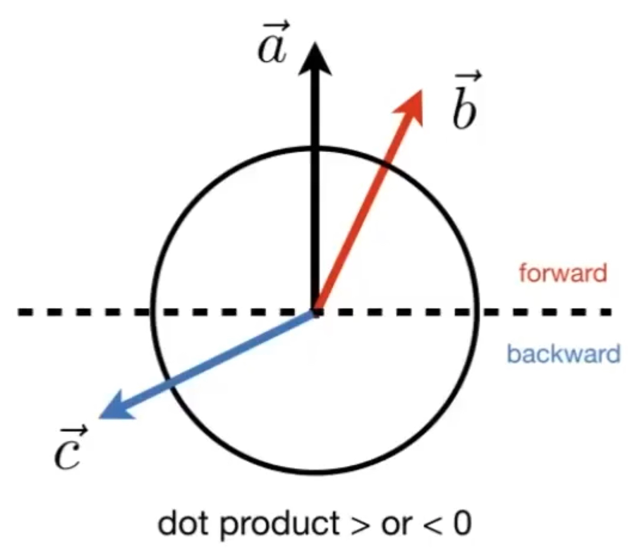
\includegraphics[scale=.25]{vectordirection.png}
		\caption{向量的方向}
		\label{fig:vectordir}
	\end{figure}

	如果两个向量方向基本相同, 那么点乘的结果大于$0$; 如果两个向量的方向基本相反, 点乘的结果小于$0$; 如果两个向量是垂直的, 那么点乘的结果等于$0$.
	
	
\end{enumerate}

\subsubsection{叉乘}

\textbf{叉乘 (Cross product) }, 又称作向量的外积. 两个向量叉乘的结果还是一个向量, 这个向量和原来的两个向量垂直. 叉乘的结果向量的长度为: 
\begin{equation}
	||a\times b||=||a||||b||\sin\phi
\end{equation}

结果向量的方向满足\textbf{右手定则}.右手定则指的是, 使用右手的四指从第一个向量到第二个向量握拳, 大拇指指向的方向是叉乘结果向量的方向. 因此叉乘不满足交换律. 

\begin{figure}[H]
	\centering
	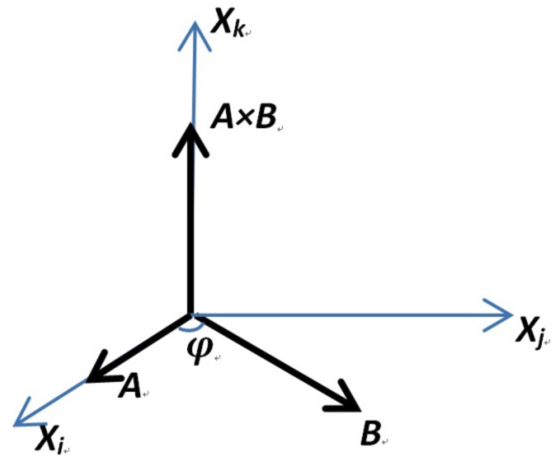
\includegraphics[scale=.25]{crossproduct.png}
	\caption{叉乘}
	\label{fig:corssproduct}
\end{figure}

叉乘满足分配律, 以及数乘结合律. 向量自己和自己的叉乘结果是0.

在笛卡尔坐标系的表示下进行叉乘计算的结果可以写作: 
\begin{equation}
	\overrightarrow{a} \times \overrightarrow{b} = \begin{pmatrix}
		y_az_b-y_bz_a\\ 
		z_ax_b-x_az_b\\
		x_ay_b-y_ax_b
	\end{pmatrix}
\end{equation}

我们可以将向量$	\overrightarrow{a}$写成等价的矩阵形式: 
\begin{equation}
	\overrightarrow{a} \times \overrightarrow{b} = 
	A*b=\begin{pmatrix}
		0&-z_a&y_a\\
		z_a& 0& -x_a\\
		-y_a & x_a & 0
	\end{pmatrix} 
	\begin{pmatrix}
		x_b\\
		y_b\\
		z_b
	\end{pmatrix} 
\end{equation}

\textbf{叉乘的应用}

\begin{enumerate}[label=1)]
	\item 判断一个向量在另一个向量的左边还是右边; 
	
	一个向量对另一个向量做叉乘, 如果说结果方向为正, 那么另一个向量在这个向量的右边. 如果结果为负, 那么在左边. 
	
	\item 判定一个点在三角形的内部还是外部. 
	\begin{figure}[H]
		\centering
		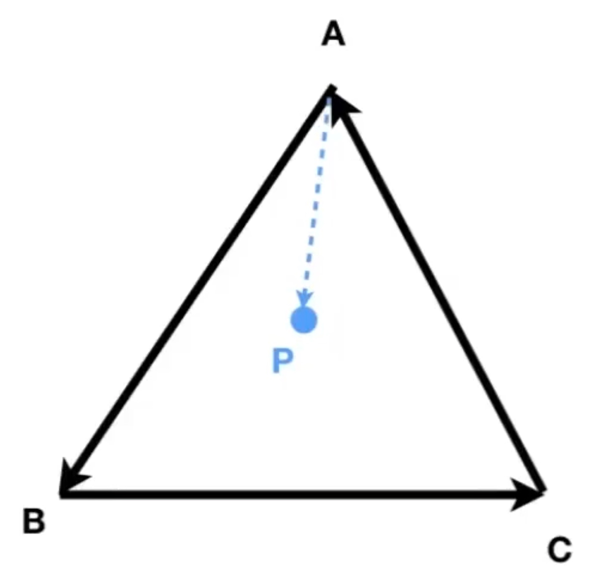
\includegraphics[scale=.25]{corssinout.png}
		\caption{判断点是否在三角形内部}
		\label{fig:corssio}
	\end{figure}

	只要P点在边AB, BC, AC (注意输入顺序) 的左边, 那么就满足P点在三角形ABC中. 那么可以对每个边分别求一次叉乘判断点是否在三角形内部. 三角形的输入必须保证为顺时针或者逆时针. 为了忽略顺时针和逆时针的差别 (顺时针输入需要要求点在三角形每一条边的右边) , 只要P在都在每条边的左边或者每条边的右边都算作在三角形内部. 对于边界情况 (如果叉乘结果为$0$) , 那么由自己根据实际问题定义这是内部还是外部. 
	
\end{enumerate}

\section{正交系/坐标系}

\textbf{右手坐标系 (right-hand system) }的定义如下. 我们定义三个坐标轴$\overrightarrow{u}$, $\overrightarrow{v}$, $\overrightarrow{w}$满足以下性质: 
\begin{equation}
	||\overrightarrow{u}||=||\overrightarrow{v}||=||\overrightarrow{w}||=1
\end{equation}

\begin{equation}
	\overrightarrow{u}\cdot\overrightarrow{v}=\overrightarrow{v}\cdot\overrightarrow{w}=\overrightarrow{u}\cdot\overrightarrow{w}=0
\end{equation}

\begin{equation}
	\overrightarrow{w}=\overrightarrow{u}\times\overrightarrow{v}\ \text{(右手定则)}
\end{equation}

那么向量$\overrightarrow{u}$, $\overrightarrow{v}$, $\overrightarrow{w}$定义了一个右手坐标系. 对于任意一个向量$\overrightarrow{p}$, 在右手坐标系中可以表示为: 
\begin{equation}
	\overrightarrow{p}=(\overrightarrow{p}\cdot \overrightarrow{u})\overrightarrow{u}+(\overrightarrow{p}\cdot \overrightarrow{v})\overrightarrow{v}+(\overrightarrow{p}\cdot \overrightarrow{w})\overrightarrow{w}
\end{equation}

\section{矩阵}

\textbf{矩阵 (Matrix) }, 是一个按照长方阵列$m\times n$排列的复数或实数集合. 

\subsection{矩阵乘法}

矩阵乘法$A\times B$必须满足$A$的列数$=B$的行数. 求出的矩阵的大小为: 
\begin{equation}
	(m\times n)(n\times p) = (m\times p)
\end{equation}

矩阵乘法不满足交换律, 但是满足结合律和分配律. 

矩阵和向量相乘时, 认为向量是一个列向量并乘在矩阵的右边. 

矩阵也有转置, 并且矩阵乘法转置满足$(AB)^T=B^TA^T$.

\textbf{单位矩阵}是一个左上到右下对角线值为$1$, 其他值为$0$的正方形矩阵, 以长度为$3$的单位矩阵为例: 

\begin{equation}
	I_{3\times 3}=\begin{pmatrix}
		1&0&0\\
		0&1&0\\
		0&0&1
	\end{pmatrix}
\end{equation}

单位矩阵定义了矩阵的逆运算. 对于矩阵$A$来说, 矩阵的逆$A^{-1}$满足: 
\begin{equation}
	AA^{-1}=A^{-1}A=I
\end{equation}

矩阵乘法的逆满足: 
\begin{equation}
	(AB)^{-1}=B^{-1}A^{-1}
\end{equation}

\chapter{变换}

\textbf{变换 (Transform) }是计算机图形学中非常重要的一部分. 变换包含模型变换 (Modeling transform) 以及视图变换 (View transform) . 模型变换指的是变换模型 (被拍摄物体) 的位置, 大小和角度; 视图变换指的是变换照相机的位置和角度. 从相对运动的角度来看, 两种变换是可以相互转化的. 

\section{模型变换}

\subsection{2维变换}

\subsubsection{缩放变换}

缩放变换 (Scale) 中, 如果一个图片以原点$(0,0)$为中心缩放$s$倍. 那么点$(x,y)$变换后数学形式可以表示为: 

\begin{equation}
\begin{split}
	x'=sx
	\\
	y'=sy
\end{split}
\end{equation}

写成矩阵形式为: 
\begin{equation}
	\begin{bmatrix}
		x' \\
		y'
	\end{bmatrix} = \begin{bmatrix}
		s&0\\0&s\end{bmatrix}\begin{bmatrix}x\\y\end{bmatrix}
\end{equation}

当然, 我们也可以给$x$轴和$y$轴不同的缩放倍数$s_x$和$s_y$. 在非均匀情况下, 缩放变换的矩阵形式为: 
\begin{equation}
	\begin{bmatrix}
		x' \\
		y'
	\end{bmatrix} = \begin{bmatrix}
		s_x&0\\0&s_y\end{bmatrix}\begin{bmatrix}x\\y\end{bmatrix}
\end{equation}

\subsubsection{反射变换}

反射变换 (Reflection) 指的是图片对着$x$轴或者$y$轴做对称变换. 对于图片上的点$(x,y)$在经过x轴的对称反射变换后, 数学形式可以表示为: 
\begin{equation}
	\begin{split}
		x'=-x\\y'=y
	\end{split}
\end{equation}

表示成矩阵形式为: 
\begin{equation}
	\begin{bmatrix}
	x' \\
	y'
\end{bmatrix} = \begin{bmatrix}
-1&0\\0&1\end{bmatrix}\begin{bmatrix}x\\y\end{bmatrix}
\end{equation}

同理可以得到$y$轴对称反射变换后的变换矩阵为: 

\begin{equation}
	\begin{bmatrix}
		x' \\
		y'
	\end{bmatrix} = \begin{bmatrix}
		1&0\\0&-1\end{bmatrix}\begin{bmatrix}x\\y\end{bmatrix}
\end{equation}

沿原点反射变换的变换矩阵为: 

\begin{equation}
	\begin{bmatrix}
		x' \\
		y'
	\end{bmatrix} = \begin{bmatrix}
		-1&0\\0&-1\end{bmatrix}\begin{bmatrix}x\\y\end{bmatrix}
\end{equation}

\subsubsection{切变变换}

\textbf{切变变换 (Shear) }, 指的是在物理学上指的是两个距离很近、大小相等、方向相反的平行力作用于同一物体上所引起的形变. 使用示意图可以更直观的去表示什么是切变. 如图\ref{fig:shear}所示, 是图片在x轴方向上发生了切变. 从图中我们可以看出所有点在y轴上的坐标不变, 在x轴上的坐标满足: $y=0$上的点, x轴坐标不发生变化; $y=1$上的点水平方向上移动了$a$个长度. 因此对于任意一个点来说, 水平方向上移动长度为$ay$. 

\begin{figure}[H]
	\centering
	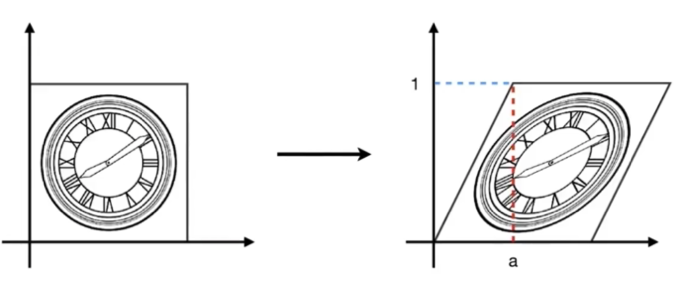
\includegraphics[scale=.25]{shear.png}
	\caption{切变变换}
\end{figure}

切变的矩阵变换可以写作: 
\begin{equation}
	\begin{bmatrix}x'\\y'\end{bmatrix}=\begin{bmatrix}1&a\\0&1\end{bmatrix}\begin{bmatrix}x\\y\end{bmatrix}
\end{equation}

\subsubsection{旋转变换*}

我们默认\textbf{旋转变换 (Rotate) }都绕着原点$(0,0)$旋转, 并且默认旋转方向为逆时针方向 (逆时针方向旋转角度值为正, 顺时针旋转角度值为负) . 旋转变换的推导过程比较复杂 (见后续推导过程) . 结论如下: 当一个点$(x,y)$绕着原单$(0,0)$旋转$\theta$角时, 变换矩阵可以表示为: 

\begin{equation}
	\begin{bmatrix}x'\\y'\end{bmatrix}=\begin{bmatrix}\cos\theta&-\sin\theta\\\sin\theta&\cos\theta\end{bmatrix}\begin{bmatrix}x\\y\end{bmatrix}
\end{equation}

\begin{titledbox}{旋转变换矩阵的推导过程}
	\begin{figure}[H]
		\centering
		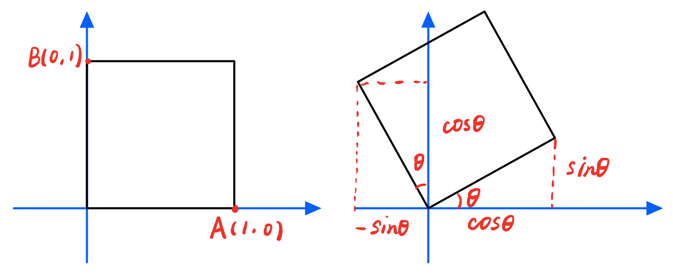
\includegraphics[scale=.25]{rotate.png}
		\caption{旋转变换的推导}
		\label{fig:shear}
	\end{figure}

我们在直角坐标系中绘制一个边长为1的正方形, 点$A$坐标为$(1,0)$, 点$B$坐标为$(0,1)$. 正方形沿着原点$(0,0)$旋转的角度为$\theta$角. 我们设: 

\begin{equation}
	\begin{bmatrix}x'\\y'\end{bmatrix}=\begin{bmatrix}A&B\\C&D\end{bmatrix}\begin{bmatrix}x\\y\end{bmatrix}
\end{equation}

代入点$A$的的值$(1,0)$可以得到: 
\begin{equation}
	\begin{bmatrix}\cos\theta\\\sin\theta\end{bmatrix}=\begin{bmatrix}A&B\\C&D\end{bmatrix}\begin{bmatrix}1\\0\end{bmatrix}
\end{equation}

解方程得到: 

\begin{equation}
\begin{split}
	A=\cos\theta\\C=\sin\theta
\end{split}
\end{equation}

代入点$B$的的值$(0,1)$可以得到: 
\begin{equation}
	\begin{bmatrix}-\sin\theta\\\cos\theta\end{bmatrix}=\begin{bmatrix}A&B\\C&D\end{bmatrix}\begin{bmatrix}0\\1\end{bmatrix}
\end{equation}

解方程得到: 

\begin{equation}
	\begin{split}
		B=-\sin\theta\\D=\cos\theta
	\end{split}
\end{equation}

因此: 
\begin{equation}
	M_{rotate}=\begin{bmatrix}\cos\theta&-\sin\theta\\\sin\theta&\cos\theta\end{bmatrix}
\end{equation}

\end{titledbox}

\subsubsection{线性变换}

对于任何一种变换如果可以写作: 
\begin{equation}
	\begin{split}
		x'=ax+by\\y'=cx+dy
	\end{split}
\end{equation}

矩阵形式可以表示为: 
\begin{equation}
	\begin{split}
	\begin{bmatrix}x'\\y'\end{bmatrix}=\begin{bmatrix}a&b\\c&d\end{bmatrix}\begin{bmatrix}x\\y\end{bmatrix}
	\\
	x'=Mx
	\end{split}
\end{equation}

那么我们认为这种变换是\textbf{线性变换 (Linear transformation) }. 

\subsection{齐次坐标}

\subsubsection{平移变换}

\textbf{平移变换 (Translation) }相比于以上的线性变换有特殊的地方. 平移变换的数学形式为: 
\begin{equation}
	\begin{split}
		x'=x+t_x\\
		y'=y+t_y
	\end{split}
\end{equation}

这种数学表示不能写作线性变换的矩阵形式, 只能记作: 
\begin{equation}
	\begin{bmatrix}x'\\y'\end{bmatrix}=\begin{bmatrix}a&b\\c&d\end{bmatrix}\begin{bmatrix}x\\y\end{bmatrix}+\begin{bmatrix}t_x\\t_y\end{bmatrix}
\end{equation}

说明平移操作\textbf{不是}线性变换. 但是我们不希望把平移操作看作特殊变换, 因此需要把这些变换统一起来, 就引入了齐次坐标. 

\subsubsection{齐次坐标的引入}

为了统一变换操作, 我们引入一个新的维度. 对于二维的点$(x,y)$我们可以增加一个维度, 对于2维的点可以表示为$(x,y,1)^T$, 2维向量的$(x,y,0)^T$. 因此, 一个点的平移可以用矩阵表示为: 
\begin{equation}
	\begin{bmatrix}x'\\y'\\w'\end{bmatrix}=\begin{bmatrix}1&0&t_x\\0&1&t_y\\0&0&1\end{bmatrix}\begin{bmatrix}x\\y\\1\end{bmatrix}=\begin{bmatrix}x+t_x\\y+t_y\\1\end{bmatrix}
\end{equation}

\begin{question}
	\textbf{为什么点补充维度大小为1, 但是向量补充维度大小为0?}
	
	对于向量来说, 平移变换不应该使向量的结果发生变化. 因此补充维度为0的时候可以屏蔽平移带来的影响. 
	
	对于加入齐次坐标的点和向量满足: 
	\begin{enumerate}
		\item 向量+向量=向量
		\item 点-点=向量
		\item 点+向量=点
		\item 点+点=\textbf{两个点中点}
		
			对引入齐次坐标的点的扩充定义如下: 
			\begin{equation}
				\begin{pmatrix}x\\y\\w\end{pmatrix}=\begin{pmatrix}x/w\\y/w\\1\end{pmatrix},w\ne 0
			\end{equation}
			因此一个点加上另一个点的结果是两个点的\textbf{中点}. 引入了扩充定义点和向量的加法是有意义的. 
	\end{enumerate}
\end{question}

\subsection{仿射变换}

\textbf{仿射变换 (Affine) }包含线性变换与平移变换. 可以用矩阵表示为: 

\begin{equation}
	\begin{bmatrix}x'\\y'\end{bmatrix}=\begin{bmatrix}a&b\\c&d\end{bmatrix}\begin{bmatrix}x\\y\end{bmatrix}+\begin{bmatrix}t_x\\t_y\end{bmatrix}
\end{equation}

使用齐次坐标后可以写作: 

\begin{equation}
	\begin{bmatrix}x'\\y'\\w'\end{bmatrix}=\begin{bmatrix}a&b&t_x\\c&d&t_y\\0&0&1\end{bmatrix}\begin{bmatrix}x\\y\\1\end{bmatrix}=\begin{bmatrix}ax+by+t_x\\cx+dy+t_y\\1\end{bmatrix}
\end{equation}

\subsection{逆变换}

任何变换的\textbf{逆变换 (Inverse transform) }的变换矩阵$M$的逆矩阵$M^{-1}$表示. 

\subsection{变换的组合与分解}

\subsubsection{变换的组合}

可以用\textbf{矩阵的乘法}进行变换的组合 (Transform compose) . 变换的先后顺序不同, 变换的结果不同. 矩阵和向量的乘法是从右到左依次相乘, 从右到左依次应用变化. 如果我们要依次应用变化$A_1,A_2,A_3,\cdots$, 写成矩阵形式: 

\begin{equation}
	A_n(\dots A_2(A_1(x)))=A_n\dots A_2\cdot A_1\cdot \begin{pmatrix}x\\y\\1\end{pmatrix}
\end{equation}

根据矩阵运算的\textbf{结合律},我们可以先把变换矩阵乘在一起, 接下来把这个矩阵的乘积和向量相乘. 可以用一个矩阵表示一个复杂的变换. 

\subsubsection{变换的分解}

所有的复杂变换都可以分解成多个普通的变换. 为了使某个图像沿着某个点$c$变换, 我们可以分解为以下步骤: 

\begin{enumerate}
	\item 把中心点$c$移动到原点; 
	\item 进行旋转; 
	\item 把中心点$c$平移到原点; 
\end{enumerate}

用变换矩阵表示为: 
\begin{equation}
	M_{t}(c)\cdot M_{r}(\theta) \cdot M_{t}(-c)
\end{equation}

\subsection{3维变换}

$3$维变换可以类比于$2$维变换得到引入齐次坐标的点和向量, $3$维的点可以表示为$(x,y,z,1)^T$, 3维向量可以表示为$(x,y,z,0)^T$. 当$w\ne 0$的时候: 
\begin{equation}
	(x,y,z,w)=(x/w,y/w,z/w,1)
\end{equation}

使用$4\times 4$的矩阵来表示仿射变换: 

\begin{equation}
	\begin{pmatrix}x'\\y'\\z'\\1\end{pmatrix}=\begin{pmatrix}a&b&c&t_x\\d&e&f&t_y\\g&h&i&t_z\\0&0&0&1\end{pmatrix}\cdot\begin{pmatrix}x\\y\\z\\1\end{pmatrix}
\end{equation}

左上角是一个$3\times 3$的线性变换矩阵. 

在仿射变换中的变换矩阵表示先\textbf{线性变换}再\textbf{平移}. 

\subsubsection{3维变换中缩放变换}
3维变换中缩放变换的变换矩阵: 
\begin{equation}
	\textbf{S}(s_x,s_y,s_z)=\begin{pmatrix}s_x&0&0&0\\0&s_y&0&0\\0&0&s_z&0\\0&0&0&1\end{pmatrix}
\end{equation}

\subsubsection{3维变换中的平移变换}
3维变换中平移变换的变换矩阵: 
\begin{equation}
	\textbf{T}(t_x,t_y,t_z)=\begin{pmatrix}1&0&0&t_x\\0&1&0&t_y\\0&0&1&t_z\\0&0&0&1\end{pmatrix}
\end{equation}

\subsubsection{3维变换中的旋转变换}

当空间内的物体绕着$x$轴, $y$轴或者$z$轴旋转的时候, 变换矩阵为: 

\begin{equation}
\textbf{R}_x(\alpha)=\begin{pmatrix}1&0&0&0\\0&\cos\alpha&-\sin\alpha&0\\0&\sin\alpha&\cos\alpha&0\\0&0&0&1\end{pmatrix}
\end{equation}

\begin{equation}
	\textbf{R}_y(\alpha)=\begin{pmatrix}\cos\alpha&0&\sin\alpha&0\\0&1&0&0\\-\sin\alpha&0&\cos\alpha&0\\0&0&0&1\end{pmatrix}
\end{equation}

\begin{equation}
	\textbf{R}_z(\alpha)=\begin{pmatrix}\cos\alpha&-\sin\alpha&0&0\\\sin\alpha&\cos\alpha&0&0\\0&0&1&0\\0&0&0&1\end{pmatrix}
\end{equation}

\begin{question}
	\textbf{为什么$\textbf{R}_y$的$\sin\alpha$的符号位置是反的?}
	
	因为只有$y$轴按照右手法则是$zx=y$, $x$轴和$z$轴的顺序是反的. 所以我规定从$z$轴到$x$轴旋转为逆时针方向的情况下, $\sin\alpha$的负号位置应该在$z$轴对应的这一行. 也可以理解为对角线上的循环移动. 
\end{question}

对于一般性的旋转问题, 可以用简单的旋转描述复杂的旋转. 用$x$轴, $y$轴和$z$轴上的旋转来定义旋转: 
\begin{equation}
	\textbf{R}_{xyz}(\alpha,\beta,\gamma)=\textbf{R}_x(\alpha)\textbf{R}_y(\beta)\textbf{R}_z(\gamma)
\end{equation}

这三个角就被称作\textbf{欧拉角 (Euler angles) }. 

\subsubsection{罗德里格斯旋转公式}

绕着旋转轴$\textbf{n}$旋转角度$\alpha$. 默认旋转轴是过原点的, 对于不过原点的条件可以将图形平移到过原点的旋转轴上, 旋转后再平移回去. 罗德里格斯旋转公式 (Rodrigues' Rotation Formula) 是: 
\begin{equation}
	\textbf{R}(\textbf{n},\alpha)=\cos(\alpha)\textbf{I}+(1-\cos(\alpha))\textbf{n}\textbf{n}^T+\sin(\alpha)\begin{pmatrix}0&-n_z&n_y\\n_z&0&-n_x\\-n_y&n_x&0\end{pmatrix}
\end{equation}

最后的矩阵一般记作$N$, 矩阵$N$满足叉乘的矩阵形式. 

%\begin{titledbox}{罗德里格斯旋转公式的证明}
%	
%	
%\end{titledbox}

\section{视图变换}

在$3$维物体变到二维平面的过程中, 我们需要规定好相机的位置. 对于相机所做的变换就是\textbf{视图变换 (Viewing/Camera transformation) }. 

\vspace{\baselineskip}
我们需要对相机位置进行定义, 对于一个相机我们要规定下面三个属性: 
\begin{enumerate}[itemsep=-0.5em]
	\item 相机位置 (Position) $\overrightarrow{e}$
	\item 相机拍摄方向 (Look-at/Gaze direction) $\hat{g}$
	\item 相机向上方向 (Up direction, 假设垂直于look-at direction) $\hat{t}$
\end{enumerate}

\vspace{\baselineskip}
根据相对运动我们可以知道, 只要相机和被拍摄物体相对位置不变, 那么拍摄出来的照片应当是一样的. 我们可以通过对被拍摄物体做相同的变换来把相机变换到标准位置. 相机的标准位置为: 
\begin{enumerate}[itemsep=-0.5em]
	\item 相机位置在原点$(0,0)$; 
	\item 相机拍摄方向是$-z$轴方向; (默认右手系)
	\item 相机的向上方向是$y$轴方向. 
\end{enumerate}

\vspace{\baselineskip}
将任意位置的相机移动到标准位置需要以下操作: 
\begin{enumerate}[itemsep=-0.5em]
	\item 将中心点$\overrightarrow{e}$移动到原点; 
	\item 把$\hat{g}$旋转到$-z$轴方向; 
	\item 把$\hat{t}$旋转到$y$轴方向; 
	\item 把$\hat{g}\times\hat{t}$旋转到$x$轴方向. 
\end{enumerate}

操作$2 \sim 4$只要满足任意两个, 另外一个条件就会满足. 也就是说我们需要先做一次平移变换, 再做一次旋转变换. 

平移变换的变换矩阵可以写作: 

\begin{equation}
	T_{view}=\begin{pmatrix}1&0&0&-x_e\\0&1&0&-y_e\\0&0&1&-z_e\\0&0&0&1\end{pmatrix}
\end{equation}

旋转矩阵的写法比较麻烦. 从$\hat{g}$旋转到$-z$轴方向, $\hat{t}$旋转到$y$轴方向以及$\hat{g}\times\hat{t}$旋转到$x$轴方向比较难写, 但是旋转变换的逆变换非常的简单: 

\begin{equation}
	R^{-1}_{view}=\begin{pmatrix}x_{\hat{g}\times\hat{t}}&x_t&x_{-g}&0\\y_{\hat{g}\times\hat{t}}&y_t&y_{-g}&0\\z_{\hat{g}\times\hat{t}}&z_t&z_{-g}&0\\0&0&0&1\end{pmatrix}
\end{equation}

我们用$x$轴方向单位向量$(1,0,0,0)$, $y$轴单位向量$(0,1,0,0)$, $z$轴单位向量$(0,0,1,0)$代入后结果是正确的. 我们知道旋转矩阵的逆矩阵是正交矩阵, 因此旋转变换矩阵的逆是旋转变换矩阵的转置矩阵. 也就是说: 

\begin{equation}
	R_{view}=\begin{pmatrix}x_{\hat{g}\times\hat{t}}&y_{\hat{g}\times\hat{t}}&z_{\hat{g}\times\hat{t}}&0\\x_t&y_t&z_t&0\\x_{-g}&y_{-g}&z_{-g}&0\\0&0&0&1\end{pmatrix}
\end{equation}

\begin{information}
	\textbf{旋转变换矩阵是正交矩阵, 矩阵的逆等于矩阵的转置. }
	
	旋转$\theta$角的逆变换就是旋转$-\theta$角. 旋转$-\theta$角的变换矩阵是: 
	\begin{equation}
		R_{-\theta}=\begin{bmatrix}\cos\theta&\sin\theta\\-\sin\theta&\cos\theta\end{bmatrix} = R_{\theta}^T
	\end{equation}

	同时: 
	
	\begin{equation}
		R_{-\theta}=R_{\theta}^{-1}\ ~ \text{(by definition)}
	\end{equation}

	旋转矩阵的逆等于旋转矩阵的转置, 这样的矩阵被称为正交矩阵. 

\end{information}

以上就是我们得到的视图变换矩阵. 

\section{投影变换}

\textbf{投影变换 (Projection transformation) }是把$3$维模型投影到$2$维平面的变换. 投影变换分为正交投影 (Orthographic projection) 以及透视投影 (Perspective projection) . 正交投影中, 投影后原本平行的线保持平行关系. 但是透视投影中平行的线在投影后不一定能保持平行关系, 会相交到某一点上 (这也就是近大远小现象) . 

\begin{figure}[H]
	\centering
	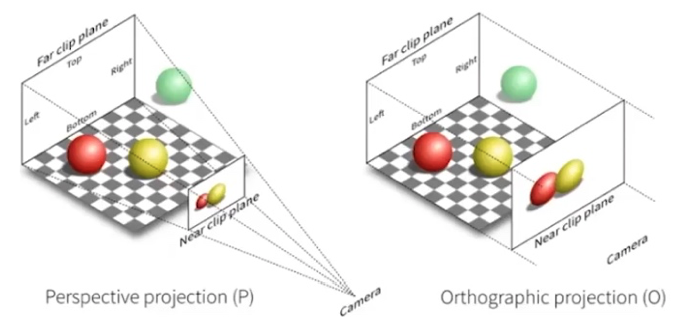
\includegraphics[scale=.4]{projection.png}
	\caption{透视投影与正交投影}
\end{figure}

\subsection{正交投影}

正交投影将相机放在原点上, 拍摄方向是$-z$轴方向, 向上方向是$y$轴方向. 只需要去掉$z$轴后, $xy$平面上的图像就是投影结果. 为了能够正交投影, 我们会把所有模型移动到$[-1,1]^3$的区间范围内. 

在空间中描述一个立方体 (立方体中包含了所有需要绘制的模型) , 将立方体变换到$[-1,1]^3$的区间范围内. 

\begin{figure}[H]
	\centering
	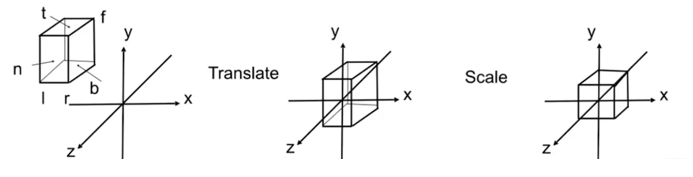
\includegraphics[scale=.4]{orp.png}
	\caption{正交投影变换}
\end{figure}

定义空间中的立方体的左右在$x$轴的坐标, 上下在$y$轴的坐标, 远近在$z$轴的坐标. 这个立方体就可以被描述$[l,r]\times[b,t]\times[f,n]$. 对于$z$轴来说, 越远$z$值更小, 越近$z$值更大. 远是小于近的, 保证了右手坐标系下从$-z$方向看过去$z$值的规律. 

将这样的立方体映射到正则/标准/规范 (canonical) 立方体$[-1,1]^3$

变换方法是先将中心平移到原点, 之后对每个边进行缩放到大小为2. 

变换矩阵为: 

\begin{equation}
	M_{ortho}=\begin{pmatrix}\frac{2}{r-l}&0&0&0\\0&\frac{2}{t-b}&0&0\\0&0&\frac{2}{n-f}&0\\0&0&0&1\end{pmatrix}\begin{pmatrix}1&0&0&-\frac{r+l}{2}\\0&1&0&-\frac{t+b}{2}\\0&0&1&-\frac{n+f}{2}\\0&0&0&1\end{pmatrix}
\end{equation}

\subsection{透视投影}

\textbf{透视投影 (Perspective projection) }是最为广泛的投影方式. 透视投影满足\textbf{近大远小}的性质. 接下来我们定义\textbf{视锥}. 视锥就是一个透视相机渲染时能看到区域的形状, 相机放在平面的中心, 一个视锥包含4个元素: 

\begin{figure}[H]
	\centering
	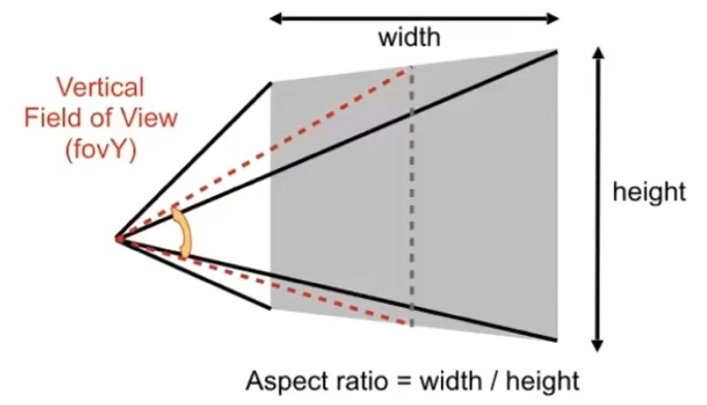
\includegraphics[scale=.3]{shizhui.png}
	\caption{视锥示意图}
\end{figure}

\begin{enumerate}[itemsep=-0.5em]
	\item 近平面: 渲染的区域里相机最近的平面; 
	\item 远平面: 渲染的区域里相机最远的平面; 
	\item 视野 (Field of view, FOV) : 平面顶部和底部中心到相机连线的夹角; 
	\item 宽高比: 平面宽度和高度之比. 
\end{enumerate}

从一个点射出的四棱锥定义了远和近两个平面. 我们可以把远平面缩小成和近平面一样大的长方形, 这样视锥就会变成一个立方体. 再做一次正交投影就可以得到最终的投影结果了. 

\begin{figure}[H]
	\centering
	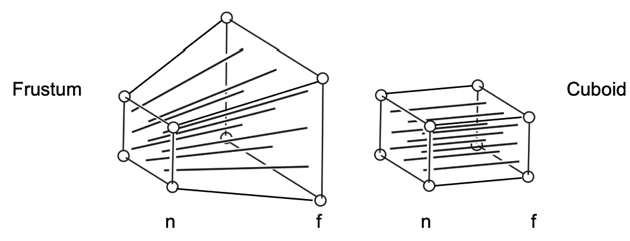
\includegraphics[scale=.4]{toushitouying.png}
	\caption{透视投影变换示意图}
\end{figure}

我们需要对这些点进行变换, 变换满足三个条件: 
\begin{enumerate}
	\item 任何一个在近平面上的点不会发生变化; 
	\item 远平面处的点z值不发生变化; 
\end{enumerate}

\begin{figure}[H]
	\centering
	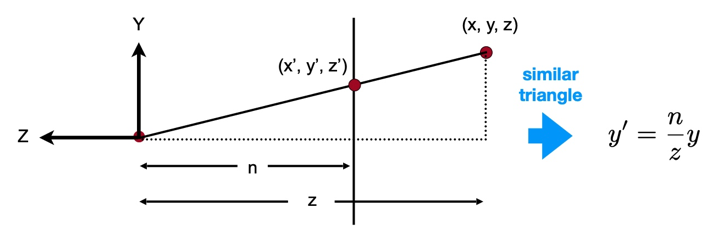
\includegraphics[scale=.4]{bianhuanjisuan.png}
	\caption{透视投影变换$YZ$平面示意图}
\end{figure}

从$YZ$平面看过去, 对于远平面上的点$(x,y,z)$在投影变换后, 根据相似三角形的性质, 点的位置变为$(\frac{n}{z}x,\frac{n}{z}y,z)$. 对于任意一个点点$(x,y,z)$来说, 变化过程为: 

\begin{equation}
	\begin{pmatrix}x\\y\\z\\1\end{pmatrix}\rightarrow\begin{pmatrix}nx/z\\ny/z\\\text{unknown}\\1\end{pmatrix}==\begin{pmatrix}nx\\ny\\\text{still unknown}\\z\end{pmatrix}
\end{equation}

中间点的$z$值变化目前是不确定的. 但是对于以上的变化结果我们可以得到变换矩阵的部分结果: 

\begin{equation}
	M_{persp\rightarrow ortho}=\begin{pmatrix}n&0&0&0\\0&n&0&0\\?&?&?&?\\0&0&1&0\end{pmatrix}
\end{equation}

接下来求出未知量. 

\textbf{此时}根据性质可知, 对于近平面上任意一点的坐标不变, 应当满足变换: \quad\textit{($n$意指$near$)}

\begin{equation}
	\begin{pmatrix}x\\y\\n\\1\end{pmatrix}\rightarrow\begin{pmatrix}x\\y\\n\\1\end{pmatrix}==\begin{pmatrix}nx\\ny\\n^2\\n\end{pmatrix}
\end{equation}

因此可以得到方程: 

\begin{equation}
	\begin{pmatrix}0&0&A&B\end{pmatrix}\begin{pmatrix}x\\y\\n\\1\end{pmatrix}=n^2
\end{equation}

$n^2$显然和$x$, $y$的值没有什么关系, 因此$x$, $y$的系数为$0$. 但是方程不能解出, 还需要一个方程. 

\textbf{这时}我们可以以利用其另外一个性质, 即远平面上任意一点的$z$坐标值不变.

对于远平面, 我们选择中心点($x$和$y$值均为$0$), 变换应当满足: \quad\textit{($f$意指$far$)}

\begin{equation}
	\begin{pmatrix}0\\0\\f\\1\end{pmatrix}\rightarrow\begin{pmatrix}0\\0\\f\\1\end{pmatrix}==\begin{pmatrix}0\\0\\f^2\\f\end{pmatrix}
\end{equation}

可以得到方程: 

\begin{equation}
	\begin{pmatrix}0&0&A&B\end{pmatrix}\begin{pmatrix}0\\0\\f\\1\end{pmatrix}=f^2
\end{equation}

方程展开后可以得到: 

\begin{equation}
	\begin{split}
		An+B=n^2\\
		Af+B=f^2
	\end{split}
\end{equation}

解得: 

\begin{equation}
	\begin{split}
		A=n+f\\
		B=-nf
	\end{split}
\end{equation}

因此我们就解出了变换矩阵: 

\begin{equation}
	M_{persp\rightarrow ortho}=\begin{pmatrix}n&0&0&0\\0&n&0&0\\0&0&n+f&-nf\\0&0&1&0\end{pmatrix}
\end{equation}

\begin{titledbox}{透视投影的变换后的正交投影变换矩阵}
	对于定义好的视锥, 我们定义视野角度为$\alpha$, 宽高比为$radio$, 近平面$z$值为$n$, 那么投影变换后的长方体的中$t=n\tan{\frac{\alpha}{2}}, b=-n\tan{\frac{\alpha}{2}}, r=radio*n\tan{\frac{\alpha}{2}},l=-radio*n\tan{\frac{\alpha}{2}}$. 代入正交投影变化公式中即可. 
\end{titledbox}

\begin{question}
	\textbf{中间点在经过透视投影变换后会变得更近还是更远? (以视锥的中间点计算为例) }
	
	计算点$(0,0,\frac{n+f}{2},1)$变换后的位置: 
	
	\begin{equation}
		\begin{pmatrix}n&0&0&0\\0&n&0&0\\0&0&n+f&-nf\\0&0&1&0\end{pmatrix}\begin{pmatrix}0\\0\\\frac{n+f}{2}\\1\end{pmatrix} = \begin{pmatrix}0\\0\\\frac{n^2+f^2}{2}\\\frac{n+f}{2}\end{pmatrix} =  \begin{pmatrix}0\\0\\\frac{n^2+f^2}{n+f}\\1\end{pmatrix}
	\end{equation}

	我们可以推算出$\frac{n^2+f^2}{n+f}\ge\frac{n+f}{2}$, 因此中间点在经过透视投影后变近了. 
\end{question}

\chapter{概率论基础}

本章内容主要介绍概率论相关基础知识, 本章数学知识将在第十三章进行使用. 

\begin{itemize}
	\item \textbf{随机变量}表示随机试验各种结果的实值单值函数, 记做$X$; 
	\item \textbf{随机变量的分布}指的是对于随机变量得到某个值的概率; 
	\item \textbf{概率}反映随机事件出现的可能性大小, 概率$p$满足: $p_i\ge 0,\sum_{i=1}^{n}p_i=1$; 
	\item \textbf{期望}指的是是试验中每次可能结果的概率乘以其结果的总和, 反映随机变量平均取值的大小; 
	\item \textbf{连续变量下的概率密度}等于一段区间(事件的取值范围)的概率除以该段区间的长度; 
	\item \textbf{连续变量的期望计算}: $E[X]=\int xp(x)dx$; 
	\item 如果$X\sim p(x)$并且$Y=f(X)$, 那么$Y$的期望为$E[Y]=E[f(X)]=\int f(x)p(x)dx$.
\end{itemize}

